\documentclass[twocolumn]{article}
\usepackage[left=0.7in,right=0.7in,top=1in,bottom=1in]{geometry}
\setlength{\columnsep}{2\columnsep}
\usepackage[utf8]{inputenc}
\usepackage{amssymb}
\usepackage{amsmath}
\usepackage{graphicx}
\usepackage[round]{natbib}
\usepackage{url}
\usepackage[pdftex,colorlinks=true]{hyperref}
\usepackage{fancyhdr}


% Define title, authors, affiliations and DOI
% ===========================================
\newcommand{\Title}{
    A better strategy for interpolating gravity and magnetic data
}
\newcommand{\Author}{
    S.R. Soler,
    L. Uieda
}
\newcommand{\AuthorAffil}{
    {\large
        S.R. Soler$^{1,2}$,
        L. Uieda$^{3}$
    }
    \\[0.4cm]
    {\small $^{1}$CONICET, Argentina (santiago.r.soler@gmail.com)} \\
    {\small $^{2}$Instituto Geofísico Sismológico Volponi, UNSJ, Argentina} \\
    {\small $^{3}$University of Liverpool} \\

}
\newcommand{\DOI}{
    doi:\href{https://doi.org/xxx.xxx/xxxxxx}{xxx.xxx/xxxxxx}
}
\newcommand{\DOILink}{
    \href{https://doi.org/xxx.xxx/xxxxxx}{doi.org/xxx.xxx/xxxxxx}
}


% Configure header and hypersetup
% ===============================
\pagestyle{fancy}
\fancyhf{}
\lhead{
    \fontsize{9pt}{12pt}\selectfont
    \Author{}, 2019. \DOI{}
}
\rhead{\fontsize{9pt}{12pt}\selectfont \thepage}
\renewcommand{\headrulewidth}{0pt}
\hypersetup{
    allcolors=blue,
    pdftitle={\Title},
    pdfauthor={\Author},
}


%%%%%%%%%%%%%%%%%%%%%%%%%%%%%%%%%%%%%%%%%%%%%%%%%%%%%%%%%%%%%%%%%%%%%%%%%%%%%%%

\begin{document}

\title{\Title}
\author{\AuthorAffil}
\date{
    \normalsize
    \today
}
\maketitle

\begin{abstract}
    My abstract
    \\[0.5cm]
    \textbf{Keywords:}
    My keywords
\end{abstract}

%%%%%%%%%%%%%%%%%%%%%%%%%%%%%%%%%%%%%%%%%%%%%%%%%%%%%%%%%%%%%%%%%%%%%%%%%%%%%%%

\section{Introduction}

Potential field data, like gravity and magnetics, are useful for geophysics
exploration.
The potential field data can be obtained from ground, airborne or satellite
measurements.
On ground surveys the data is often gathered on scattered points or following
irregular paths, usually at the topographic surface.
The data points have different heights.
On airborne surveys the data is gathered on flight paths, producing a large
number of data points concentrated along almost straight lines.
The height of measurement could change because of the vertical movement of the
airship.
To improve visualization of the data for interpretation and to prepare the data
for processing through different methods (RTP, upward continuation, Euler
deconvolution, etc), the data needs to be interpolated on a regular grid of
data points.

There are several methods for interpolating 2D data like minimum curvature,
biharmonic Splines or Kriging.
These all-purpose methods show a few problems when applied to potential field
data.
(i) They don't take into account the height of the observation points.
Potential field data has a strong dependency on measurement height.
(ii) The predicted grid data is not necessary an Harmonic function.
(iii) They don't usually take into account the anisotropy of the observation
points in ground and airborne surveys.

One of the most widely used methods for interpolating gravity and magnetic data
is the equivalent sources technique (also known as equivalent layer, radial
basis functions or Green's functions interpolation).
It consists in estimating a source distribution that produces the same field as
the one measured and using this estimate to predict new values.
\citet{dampney1969} was the first to introduce the equivalent source technique.

The EQL can be used for interpolation of potential field data
\citep{cordell1992, cooper2000}.
It has been also used for applying a reduction to the pole to magnetic data
\citep{guspi2009, silva1986, emilia1973, nakatsuka2006} or an upward
continuation (cite).

The most widely used source distribution is a set of point sources.
The potential field of point sources is easy to compute.
\citet{barnes2011} make use of prisms.
How to locate these point masses?
Existing approaches:
(i) one point source beneath each observation point at a constant depth (cite),
(ii) one point source beneath each observation point at a depth proportional to
the distance to its nearest data points (cite),
(iii) a regular grid of sources \citep{barnes2011}.

We want to find out which distribution of sources produces the best
interpolations.


%%%%%%%%%%%%%%%%%%%%%%%%%%%%%%%%%%%%%%%%%%%%%%%%%%%%%%%%%%%%%%%%%%%%%%%%%%%%%%%

\section{The equivalent sources technique}

The Green's equivalent layer theorem states that any harmonic potential field
generated by any three dimensional physical-property distribution can by
reproduced by a continuous two dimensional surface distribution.
This introduces an ambiguity on the distribution that generates
a potential field: multiple physical-property distributions can generate the
same potential field.
This represents an obstacle for determining the true shape and
physical-property distribution that generates any measured potential field.
Nevertheless this ambiguity can also be exploited for developing preprocessing
techniques like interpolating potential field data.

Approximating the continuous distribution by a finite and discrete density
distribution is the basis of the \emph{equivalent sources technique}
\citep{dampney1969}.
The most common approach is to make use of a set of point sources (the
\emph{equivalent sources}) located beneath the observation points.

A classical approach for applying the equivalent sources technique would be to
propose a set of point sources that generate the same harmonic field that has
been measured.
Lets consider a set of gravity acceleration measurements $g_z$ on points
$\{\mathbf{p}_1, \ldots, \mathbf{p}_N\}$ and a set of point sources with mass
$\{m_1, \ldots, m_M\}$ located on points
$\{\mathbf{q}_1, \ldots, \mathbf{q}_M\}$.
The point sources must generate the same gravity field as the one measured:

\begin{equation}
    g_z(\mathbf{p}) = \mathbf{A} \mathbf{m},
    \label{eq:linear-problem-g}
\end{equation}

\noindent where $g_z(\mathbf{p})$ is the vector containing the measured
field on the points $\mathbf{p}$, $\mathbf{m}$ is the vector containing the
masses of the point sources and $\mathbf{A}$ a matrix whose
elements can be obtained as the vertical component of the gravitational
acceleration measured on $\mathbf{p}$ due to the point mass on $\mathbf{q}$:

\begin{equation}
    a_{ij} = G \frac{(z_i - z_j)}{|\mathbf{p}_i - \mathbf{q}_j|^3},
\end{equation}

\noindent where $z_i$ and $z_j$ are the vertical components of the
$\mathbf{p}_i$ and $\mathbf{q}_j$ points, respectively.

By solving equation~\ref{eq:linear-problem-g} we can obtain the values of
$\mathbf{m}$ that better reproduce the measured field.
This source distribution along with the fitted masses can be used to predict
gravity values on any point where the potential field has not been measured.


\subsection{Generalization of equivalent sources}

It's possible to generalize the equivalent sources technique to any harmonic
field through a Green's function problem, regardless the nature of the field.

By definition, any harmonic field $V$ must satisfy the Laplace's equation:

\begin{equation}
    \nabla^2 V = 0.
\end{equation}

The fundamental solution $\psi$ \citep[p.~210]{vladimirov1979} of the harmonic
field $V$ must satisfy:

\begin{equation}
    \nabla_\mathbf{p}^2 \psi(\mathbf{p}, \mathbf{q}) =
        - 4\pi \delta(\mathbf{p}, \mathbf{q})
\end{equation}

\noindent where $\delta(\mathbf{p}, \mathbf{q})$ is the Dirac's delta function
and $\nabla_\mathbf{p}$ symbolize the Nabla operator applied on the
coordinates $\mathbf{p}$.

Assuming that $\psi$ tends to zero when approaching to infinity as boundary
condition, the fundamental solution of any harmonic field can be obtained as
follows \citep{blakely1995}:

\begin{equation}
    \psi(\mathbf{p}, \mathbf{q})
    =
    \int
    \frac{\delta(\mathbf{p}, \mathbf{q})}{|\mathbf{p} - \mathbf{q}|}
    \textrm{d}v
    =
    \frac{1}{|\mathbf{p} - \mathbf{q}|}.
\end{equation}

This shows that the Green's function associated with any harmonic field is
equal to the inverse of the Cartesian distance between the evaluation and the
source points.
Thus any harmonic field $V$ can be expressed as \citep[p.~37]{blakely1995}:

\begin{equation}
    V(\mathbf{p})
    =
    \int \psi(\mathbf{p}, \mathbf{q}) \rho(\mathbf{q}) d\mathbf{q}
    =
    \int \frac{\rho(\mathbf{q})}{|\mathbf{p} - \mathbf{q}|}  d\mathbf{q},
\end{equation}

\noindent where $\rho(\mathbf{q})$ is the density distribution of a certain
physical-property evaluated on the point $\mathbf{q}$. Following
\citet{dampney1969}, this density distribution can be approximated by a finite
and discrete set of point sources located on $\{\mathbf{q}_1, \ldots,
\mathbf{q}_M\}$:

\begin{equation}
    \rho(\mathbf{q}) =
        \sum\limits_{j=1}^{M} c_j \delta(\mathbf{q} - \mathbf{q_j}),
\end{equation}

\noindent where $c_j$ is a coefficient related to the point source located on
$\mathbf{q}_j$, with the same units as the physical-property.
Then the harmonic field $V$ can be approximated by:

\begin{equation}
    V(\mathbf{p})
    =
    \sum\limits_{j=1}^{M} \frac{c_j}{|\mathbf{p} - \mathbf{q}_j|}.
    \label{eq:eql-field}
\end{equation}

In case we have measured the value of the harmonic field on points
$\{\mathbf{p}_1, \ldots, \mathbf{p}_N\}$, we can adjust the values of the $c$
coefficients so they satisfy:

\begin{equation}
    V(\mathbf{p}_i)
    =
    \sum\limits_{j=1}^{M} \frac{c_j}{|\mathbf{p}_i - \mathbf{q}_j|}
    \quad \forall i=1,\ldots,N.
\end{equation}

This system of linear equations can be written in an more algebraic way:

\begin{equation}
    V(\mathbf{p}) = \mathbf{A} \mathbf{c}
    \label{eq:linear-problem}
\end{equation}

\noindent where $V(\mathbf{p}$) is a vertical vector containing the measured
values of $V$ on the observation points, $\mathbf{c}$ a vertical vector
containing the $c$ coefficients and $\mathbf{A}$ is the \emph{Jacobian matrix},
whose elements are defined as the Green's function evaluated on each pair of
points $\mathbf{p}$ and $\mathbf{q}$:

\begin{equation}
    a_{ij}
    =
    \psi(\mathbf{p}_i, \mathbf{q}_j)
    =
    \frac{1}{|\mathbf{p}_i - \mathbf{q}_j|}
\end{equation}

By solving equation~\ref{eq:linear-problem} we can obtain the values of
$\mathbf{c}$ that better reproduce the measured field.
Then they can be used to predict the value of the harmonic field on any other
point where no measurement has been taken by evaluating
equation~\ref{eq:eql-field}.

Worth noting that solving equations~\ref{eq:linear-problem-g}
and~\ref{eq:linear-problem} is equivalent to performing an inversion and thus
solving an ill-posed problem by nature due to the non-uniqueness and the
instability of the possible solutions.
Therefore is usually needed to add regularization functions in order to obtain
stable solutions \citep{oliveira2013}.
Moreover there's no limitation on the amount of point sources.
The number of sources can either be equal, less or more than the number of
observation points, leading to well, under or overdetermined linear problem,
respectively.

% Add other possible applications to the EQL like RTP or upward continuation.

% EQL implementation on Harmonica.

\subsection{Equivalent sources implementation}

The subsequent comparisons between strategies for interpolating data through
equivalent sources are carried out by the equivalent sources implementation in
Harmonica \citep{harmonica}.

It solves equation~\ref{eq:linear-problem} by a least-squares fit, with
the option of adding a zeroth-order Tikhonov \citep{tikhonov} regularization
through a dimensionless \emph{damping} parameter.
This is achieved by scaling the Jacobian matrix so each column has unit
variance.

Define a diagonal matrix $S$, whose elements corresponds to the standard
deviation of each column of the Jacobian matrix $\mathbf{A}$:

\begin{equation}
    \mathbf{S} =
    \begin{bmatrix}
        \sigma_1 & \cdots &0 \\
        \vdots & \ddots & \vdots \\
        0 & \cdots & \sigma_M
    \end{bmatrix}.
\end{equation}

Equation~\ref{eq:linear-problem} can be written as:

\begin{equation}
    V(\mathbf{p})
    =
    \mathbf{A} \mathbf{S}^{-1} \mathbf{S} \mathbf{c}
    =
    \left[
        \mathbf{A} \mathbf{S}^{-1}
    \right]
    \left[
        \mathbf{S} \mathbf{c}
    \right]
    =
    \mathbf{A}' \mathbf{c}'
\end{equation}

\noindent where $\mathbf{A}'$ the scaled Jacobian matrix and $\mathbf{c}'$ is
a vector containing scaled coefficients.

Now we can define the misfit function as the sum between the data misift and
the Tikhonov regularization function:

\begin{equation}
    \phi(\mathbf{c'}) =
        \left\lVert V(\mathbf{p}) - \mathbf{A}'\mathbf{c}' \right\rVert ^ 2
        + \lambda \left\lVert \mathbf{c}' \right\rVert ^2,
    \label{eq:misfit}
\end{equation}

\noindent where $\lambda$ is a dimensionless damping parameter.

After solving the least squares problem, we obtain the set of scaled
coefficients $\mathbf{c}'$ that minimizes equation~\ref{eq:misfit}.
We can get the corresponding coefficients $\mathbf{c}$ by rescaling
$\mathbf{c}'$:

\begin{equation}
    \mathbf{c} = \mathbf{S}^{-1} \mathbf{c}'.
\end{equation}



%%%%%%%%%%%%%%%%%%%%%%%%%%%%%%%%%%%%%%%%%%%%%%%%%%%%%%%%%%%%%%%%%%%%%%%%%%%%%%%

\section{Source distributions}

% Describe the proposed source distributions as combination of layouts and
% depths strategies.

The choice of a source distribution is not trivial and plays an important role
on the accuracy of the predictions.

The most widely used source distributions are: a regular grid of point sources
and one point source beneath each observation point.

The \emph{regular grid} creates an homogeneous distribution of point sources
bellow the surveyed region.
It could create too many sources on areas without data and very few ones on
areas with a high number of observation points, leading to an underfitting of
the observed data.
This could be solved by reducing the grid spacing and therefore increasing the
number of point sources and the computational load of the interpolation
process.

The \emph{source beneath data} layout adds sources where they are more needed.
If the survey is composed by a large number of data points clustered on paths
(like an airborne survey), putting one source beneath each observation point
will create an anisotropic source distribution: there will be several sources
distributed along a privileged direction.
This could introduce aliases on the predictions and increase the computational
load for fitting the predictor.

We propose a new source distribution that could simultaneously solve the
problems of the preceding ones: the \emph{block-median sources}.
It consist in dividing the region in blocks of equal size, computing the median
location of the observation points that fall inside each block, and putting one
point source bellow this block-median coordinate.
It creates one point source beneath each populated block, solving the problem
of the \emph{grid sources} layout, but also reducing the number of point
sources in comparison with the \emph{source beneath data} layout.

The depth of the point sources can be chosen following different criteria.
Deep sources generate low frequencies, while shallow ones generate high
frequencies (cite).
The most simple option is to locate all point sources at the same depth, which
we will call \emph{constant depth} in the future.
If the measurement where taken at significantly different altitudes, the
elevated computation points will be more distant to the sources than the lower
ones.
This may create problems on reproducing high frequencies on the elevated
points.

One possible solution is to locate each source bellow its corresponding
observation point or block-median point at a constant \emph{relative depth}
from it.
The sources won't be all at the same depth, but they will all be at the same
distance from their corresponding observation point or block-median point.
It worth mention that this approach could not be applied to \emph{grid
sources}.

In case our survey presents heavily clustered data points, we may want to
reduce the depth of the sources bellow that region in order to reproduce the
high frequencies measured by these clustered observation points.
We can propose a \emph{variable relative depth} approach that locates each
point source to a depth proportional to the mean distance to its $k$ nearest
source neighbours \citep{cordell1992, guspi2004, guspi2009}.
We propose to add a static shift to the computed depth in order to prevent very
shallow sources in case the mean distance to the $k$ nearest neighbours is too
small.
In summary, the depth of the sources can be set as follows:

\begin{equation}
    \textrm{depth} =
        \textrm{depth factor} \cdot \textrm{mean distance}
        + \textrm{static shift}
\end{equation}

\noindent where the \emph{depth factor} and the \emph{static shift} are
parameters and the \emph{mean distance} is the mean distance to the $k$
nearest source neighbours.

\begin{figure*}
    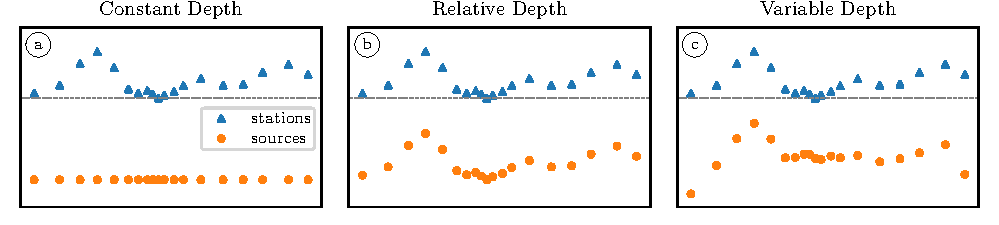
\includegraphics[width=\linewidth]{figs/depth_types.pdf}
    \caption{Cartoon illustrating the different depth types.}
    \label{fig:depth-types}
\end{figure*}


The combination of the three source layouts with the three strategies to define
the depth of the sources define seven different source distributions (see
Table~\ref{tab:source-distributions}).
The \emph{grid sources} is only compatible with the \emph{constant depth}
scheme.


\begin{table*}
\begin{minipage}{80mm}
    \caption{
        Source distributions as combinations of source layouts and depth
        strategies.
    }
    \label{tab:source-distributions}
    \begin{tabular}{lccc}
        & Source bellow data & Block-median sources & Grid sources \\ \hline
        Constant depth          & $\checkmark$ & $\checkmark$ & $\checkmark$ \\
        Relative depth          & $\checkmark$ & $\checkmark$ & $\times$     \\
        Variable relative depth & $\checkmark$ & $\checkmark$ & $\times$     \\
    \end{tabular}
\end{minipage}
\end{table*}


%%%%%%%%%%%%%%%%%%%%%%%%%%%%%%%%%%%%%%%%%%%%%%%%%%%%%%%%%%%%%%%%%%%%%%%%%%%%%%%

\section{Comparison of source distributions}

Compare the accuracy of the predictions made by each source distribution.
Need an objective way to compare them.
Propose a synthetic gravity model made out of prisms of different sizes and
density contrasts.
Create a regular grid of observation points where the gravitational effect of
the synthetic model will be computed.
Call it the \emph{target grid}.
Generate synthetic surveys above the same synthetic model and compute the
gravitational effect of the model on each survey.
Use each source distribution to predict values based on the ones obtained on
each survey onto the same grid points of the \emph{target grid}.
Score each interpolation by comparing the predicted values with the
\emph{target grid}.
Finally compare the accuracy of the predictions made by each source
distribution.

\subsection{Synthetic Model}

Describe forward model made out of prisms.
Show prisms model?

\subsection{Synthetic Surveys}

Create synthetic surveys to produce observation points.
In order to compare each source layout under very different set of observation
points we create a ground and an airborne synthetic surveys.
We selected a portion of the Southern Africa Gravity Data obtained by Dr. R.J.
Kleywegt et al.\ and made available through the NOAA website
(\url{https://www.ngdc.noaa.gov/mgg/gravity/gravity.html}) for creating
a synthetic ground survey.
We selected a portion of the Great Britain Aeromagnetic Survey acquired by
Hunting Geology and Geophysics Ltd and Canadian Aeroservices Ltd between 1955
and 1965 and made available by the
\href{
    https://www.bgs.ac.uk/products/geophysics/aeromagneticRegional.html
    }{
    British Geological Survey (BGS)
}
, for creating a synthetic airborne survey.

The gravitation effect of the synthetic model has been computed on both surveys
and added Gaussian noise (standard deviation of 1mGal) to simulate acquisition
errors.

\subsection{Comparisons}

%Describe the target grid. Show target grid figure.
%Describe the parameters used for each source distribution, how do we score
%each interpolation.
%Describe the Harmonica implementation of the EQL.
%Show results.

Compute the gravitational effect of the synthetic model on a regular grid of
points located at the same height.
This will be called our \emph{target grid}.
We will use it to compute the accuracy of the predictions made by each source
distribution.

Take a source distribution, fit the source coefficients and then use them to
predict data on the grid points where the \emph{target grid} is defined.
Define prediction error as the difference between the predicted values and the
\emph{target grid}.

Each source distribution has parameters that need to be specified before
fitting its coefficients.
For example, the \emph{grid of sources} needs the depth at which the sources
will be located.
The damping parameter used on the fitting process must also be specified
beforehand.
These parameters play an important role on the accuracy of the prediction.
We compute several predictions made by the same source distribution, but with
different values for its parameters.
Then we score each interpolation by computing the R$^2$ between each prediction
and the target grid.
We keep the best prediction, i.e.\ the one that has the highest R$^2$ score.

%%%%%%%%%%%%%%%%%%%%%%%%%%%%%%%%%%%%%%%%%%%%%%%%%%%%%%%%%%%%%%%%%%%%%%%%%%%%%%%

\section{Discussion}

%%%%%%%%%%%%%%%%%%%%%%%%%%%%%%%%%%%%%%%%%%%%%%%%%%%%%%%%%%%%%%%%%%%%%%%%%%%%%%%

\section{Conclusions}

%%%%%%%%%%%%%%%%%%%%%%%%%%%%%%%%%%%%%%%%%%%%%%%%%%%%%%%%%%%%%%%%%%%%%%%%%%%%%%%

\section{Acknowledgements}

We are indebted to the developers and maintainers of the open-source software
without which this work would not have been possible.

%%%%%%%%%%%%%%%%%%%%%%%%%%%%%%%%%%%%%%%%%%%%%%%%%%%%%%%%%%%%%%%%%%%%%%%%%%%%%%%

\bibliographystyle{plainnat}
\bibliography{references}

\end{document}
